\documentclass[12pt]{article}
\usepackage[utf8]{inputenc}
\pagenumbering{Roman}
\usepackage{ragged2e}
\usepackage{graphicx}
\usepackage{wrapfig}

\title{\huge Perfect Dream11 Team}
\author{Karthik R Prakash \\ Ravikant Yadav \\ Rajat Bhakoria \\}
\date{\today}

\begin{document}

\maketitle
\newpage
\tableofcontents
\newpage

\section{Introduction}

\justifying
Cricket is a game played and loved by many in the Indian Subcontinent. It has become so popular that it does not only dominate sports, but also as a fantasy sport in the form of applications.\par
One of these applications is Dream11. Played by many in India, this app allows cricket fans to create their own cricket team in a match using players from both sides. This project allows users to get a prediction of a good Dream11 team, by observing the past individual scores of each player. These individual scores will depend on various factors under which the match was held like date, venue, opponent team players of the match.\par
This user manual provides is a comprehensive guide to the user on how to use the website \textit{Perfect Dream 11}. It includes the functionalities that the user can experience, and detailed guidance on how to use these functionalities. The project has various use cases which are described in later sections, like, \textit{Sign Up} use case, \textit{Login} use case, \texit{prediction} use case.\par
The first section provides a brief introduction to all the functionalities/use cases in the web application. It will also explain all the web pages that are included as part of the application.\par
The second section will give the user a detailed view of what each functionality is and how to use it. These details will not include the internal workings of the web application, but will be enough for the user to use every use case of the application.\par

\newpage
\section{Motivation}
The primary problem that is faced by the management of any cricket team is the selection of good cricket players for any match. The selection of every player, right upto the selection of the extras decides the outcome of the game. Moreover since the feelings of many cricket fans is attached with how the game goes, it is very important for the management team to be precise.\par
With so many stake holders, and so many factors deciding the selection of a good cricket team, it is vital that the process for the selection not be manual, but rather automated in some sense. Also since there is no deterministic way of determining a perfect team, there should also be some softness associated with this automation.\par
Using the above arguments it is imperative for us to use a machine learning approach in order to predict such a team. This project applies these approaches to the fantasy sport of Dream11.\par
The objective of this project is to make the decision taking task of selecting a good team easier. Dream11 is used as a site to test these automation techniques, making it attractive for the common cricket fan to use it.\par

\newpage
\section{Functionalities}
\subsection{Home Page}
This page will contain public information related to all the matches that are about to be played. These are the matches on which the user can run predictions. This page also shows some information about the page, developers. The page also contains options to sign up, login, and show the list of players playing in each individual match.\par
This page is the page from where a user can navigate to every other use case of the web application.\par
%%%%%%%%%%%%%%%%%%%%%%%%%%%%%%%%%Insert image here%%%%%%%%%%%%%%%%%%%%%%%%%%%%%%%%%%%
\subsection{Player Details}
On the home page once the user clicks on a match which is about to be held, the user can see the list of players that are playing in the match. These details also contain the list of batsmen, bowlers, wicket keepers, and all rounders playing in the match. Along with the name of the players, the credit score of each player is also displayed. This credit score is proportional to the performance and experience of each player.
\subsection{Sign Up}
This functionality allows the user to sign up with the website, and allows the web application to provide the predict Dream11 team to only those users who are authenticated correctly. The sign up only asks for the \textbf{email address} of the user and the \textbf{password}.
\subsection{Login}
Once the user has signed up, the user can then log into the web application to use services like prediction of a perfect team.
\subsection{Prediction}
This user can use this functionality to predict a good Dream11 team of that match. This functionality uses a pre trained machine learning model for its prediction. The prediction is made using the individual scores of each player as determined by the ML model on the server.\par

\newpage
\section{Use Cases}
This section describes in detail each use case of the web application.

\subsection{Home Page}
This functionality is the default functionality when the user opens the website. It works the same for authenticated and unauthenticated users. On opening the website the page shows a list of upcoming matches. The home page also shows details about the website, the authors, and a space where the user can contact the website management for suggestions or complaints.\par
The home page also contains a menu bar, from where we can use the functionalities,
\begin{itemize}
    \item Contact Us: Navigates to the \textit{Contact Us} use case.
    \item Close: Closes the menu bar.
    \item Login: Navigates to the \textit{Login} use case.
    \item About Me: Navigates to the \textit{About Me} use case.
\end{itemize}
\begin{figure}[!h]
    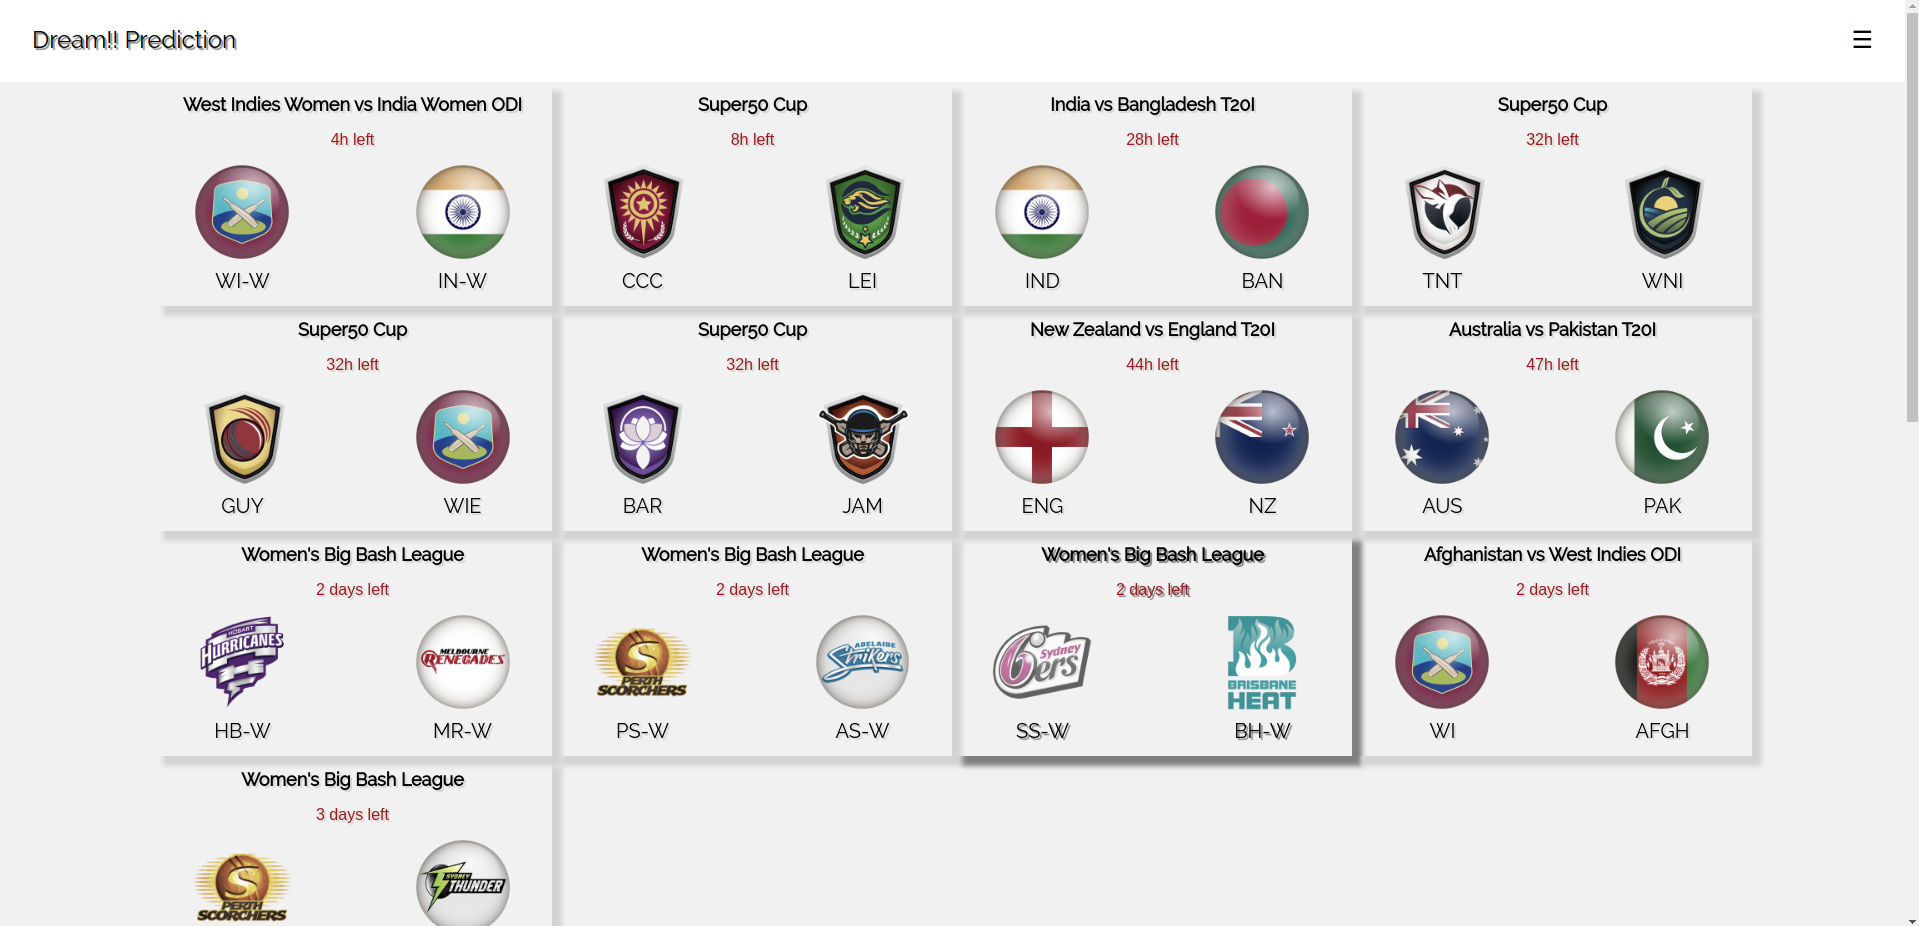
\includegraphics[scale=0.2]{homepage.png}
    \caption{Login use case}
\end{figure}
\par The matches displayed on the home page displays the following information of the match,
\begin{itemize}
    \item Team Names
    \item Tournament Name
    \item Logos of teams
    \item Time left till the match begins
\end{itemize}

\begin{center}

\begin{table}[!h]
\begin{center}
\begin{tabular}{ c c }
    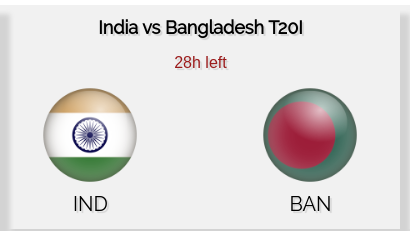
\includegraphics[height=3.6cm,width=5.3cm]{match.png} & 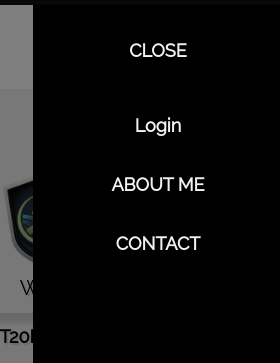
\includegraphics[height=3.6cm,width=5.3cm]{menubar.png}\\
    
\includegraphics[height=3.6cm,width=5.3cm]{aboutus.png} &         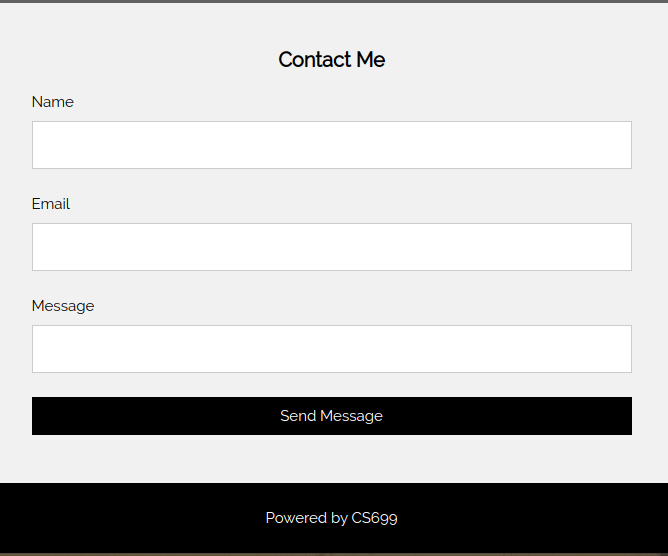
\includegraphics[height=3.6cm,width=5.3cm]{contactme.png}
\end{tabular}
\caption{Functionalities on the homepage}
\end{center}
\end{table}
\end{center}

\subsection{Login}
This functionality will allow the user to authenticate themselves with the web server. In order to navigate to this functionality, the user needs to click on the \textit{Login} option on right hand side menu bar.\par
On clicking, a CSS animation pops up, asking the user to fill in their credentials to login to their account. If an account does not exist the user may also choose to create one using the \textit{Sign Up} button.
\begin{figure}[!h]
\begin{center}
    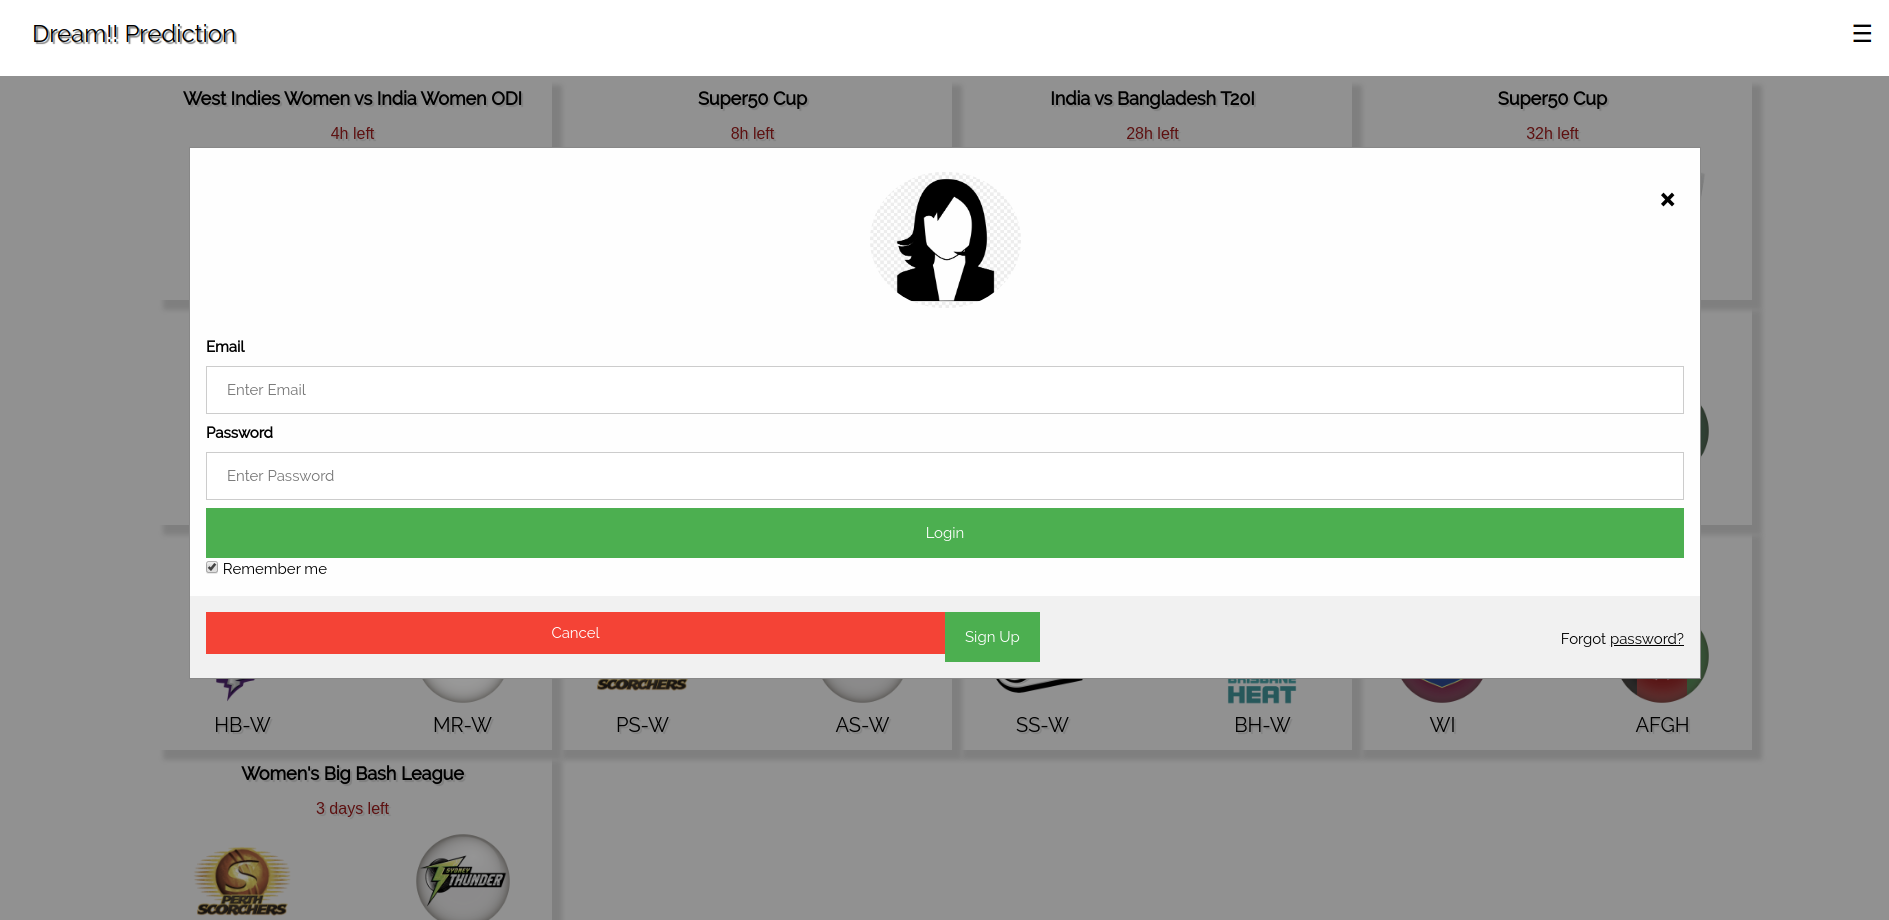
\includegraphics[scale=0.2]{login.png}
\end{center}
    \caption{Login use case}
\end{figure}


\subsection{Sign Up}
This functionality allows the user to sign up with the web application. This information can be used by the web application in the future to authenticate the user. Since only authenticated users can use some functionalities of the application, this use case is vital to the web application.

\begin{figure}[!h]
\begin{center}
    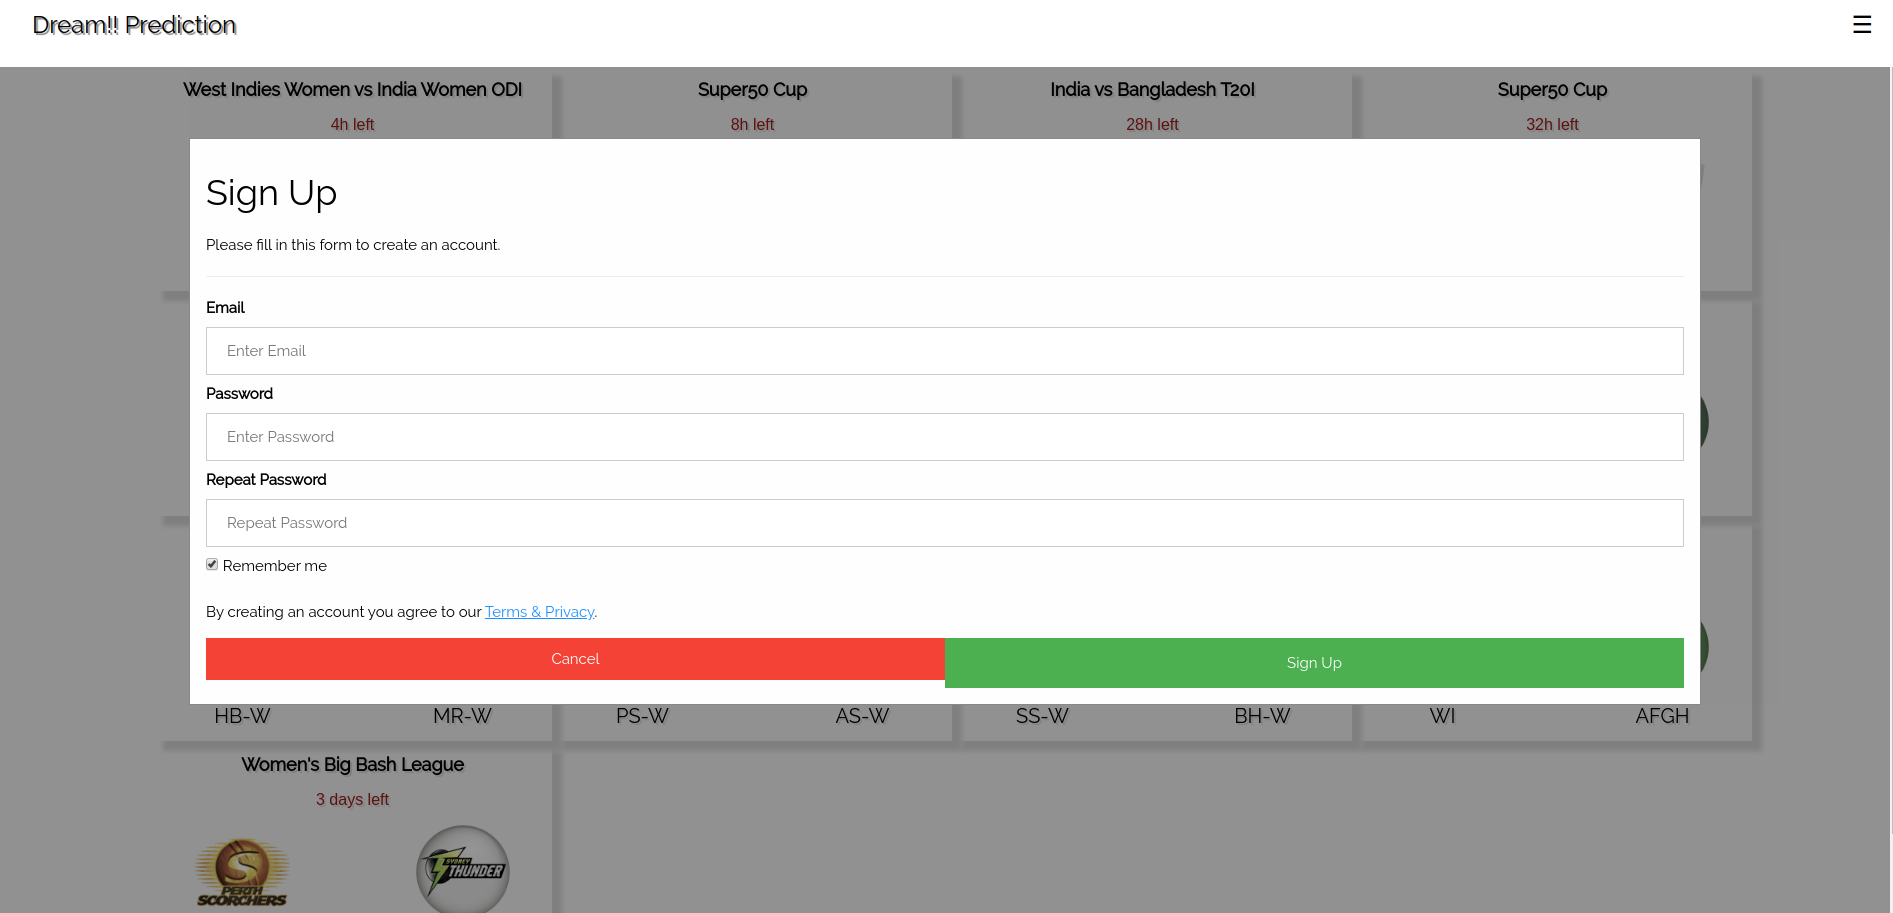
\includegraphics[scale=0.2]{signup.png}
\end{center}
    \caption{Sign Up use case}
\end{figure}
\par For using this use case the user needs to first click on the \textit{login} button on the side menu bar. After this the login use case is opened up, with two buttons on the bottom,
\begin{itemize}
    \item Login: To be used for the \textit{login} functionality
    \item Sign Up: To be used for the \textit{sign up} functionality
\end{itemize}
In this if the user clicks on the \textit{Sign Up} button, and fills in the details required, the user can then register themselves with the web application.

\subsection{Player Details}
\par This use case will display details of a particular match in greater detail right upto the list of batsmen, bowlers, wicket keepers, and all rounders playing in the match. In order to navigate to this use case, the user just needs to click on a match.
\par The functionality will display the list of players playing in that match split according to their category. It will also display the credit score of each player, as assigned by Dream11.
\begin{figure}[!h]
    \begin{center}
        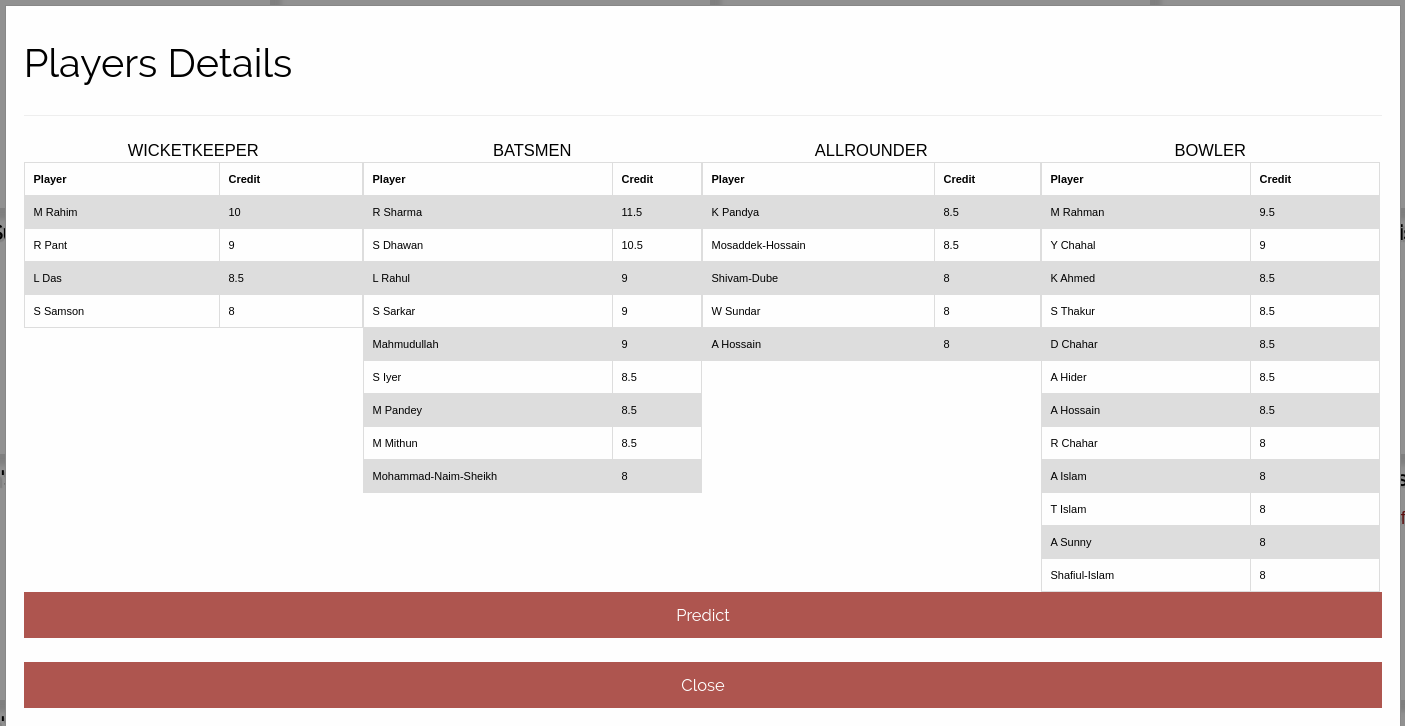
\includegraphics[scale=0.2]{playerdetails.png}
    \end{center}
    \caption{Player Details use case}
\end{figure}
\par The user can also run the \textit{Prediction} use case over here, given the user is already logged in.
\par If the user is not logged in the application will prompt the user to login to the website first.

\subsection{Prediction}
\par This functionality is the main part of the web application which provides the predicted score of each player playing in the match selected by the user. To navigate to this functionality, the user needs to be in the \textit{Player Details} use case.
\begin{figure}[!h]
    \begin{center}
        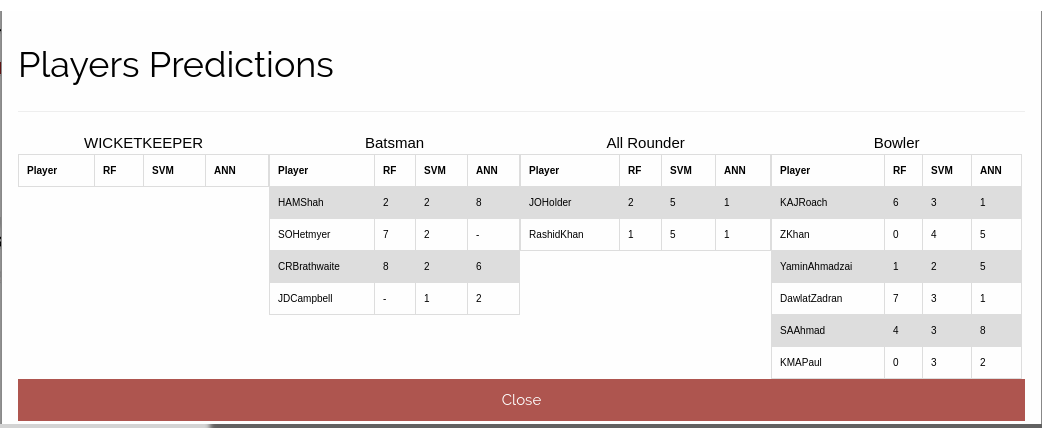
\includegraphics[scale=0.2]{prediction.png}
    \end{center}
    \caption{Prediction use case}
\end{figure}
%%%%%%%%%%%%%%%%%%%%%%%Insert Prediction use case here%%%%%%%%%%%%%%%%%%%%%%%%%%%%%%%%%%%%%%%%%
\newpage
\section{Technologies used}
\begin{itemize}
    \item HTML/CSS: Used in Developing front-end of the website.
    \item Java Script:Used in Login/SignUp Page 
    \item Web Scraping: Beautiful Soup is used to fetch the data of upcoming matches
    \item Python: Back-end is fully written in Python
    \item Keras: Python Framework used to train and predict score of each player.
    \item Doxygen: Developer Manual is generated by the help of it.
    \item Latex: User Manual is developed using it.
\end{itemize}

\newpage

\section{Future Project Application}
This project was designed to make prediction of player performance more efficient and automated. This was then used to predict a good Dream11 team, for making it more attractive for the common user. By predicting player performance based on previous matches, the project can find applications in many different domains.
\par By using the core prediction functionality, the project can be used to determine a good set of players among variety of sports such as: Foot Ball, Basket Ball, Hockey, Kabbadi which are currently hosted by Dream11.
\par There are enormous of other websites like Dream11 which allows users to play fantasy leagues, and this Project will directly help in playing at those websites to predict the perfect team. Thus increasing the end users of this project/website.




\end{document}

